\subsection{Connected Component}
After executed connected component algorithm on the cit-Patents dataset, we found that there are 3627 components in the graph, and the size of the biggest component is 3764117. \\
\\
For soc-Epinions1 dataset, we found that there are 2 components in the graph, and the sizes of components are 75877 and 2. \\
\subsection{Eigenvalue}
cit-patent:\\
\begin{tabular}{ l r }
1 & 53.64209492\\
2 & 10.32982762\\
3 & -5.606214201\\
\end{tabular}
\\
soc-Epinions1:\\
\begin{tabular}{ l r }
1& 241.4042149\\
2 & 17.96681342\\
3 & -14.38048991\\
\end{tabular}
\subsection{K core}
After executed 5-core algorithm on the cit-Patents dataset, we found that there are three 5-cores components in the graph, and the sizes of components are 1847127, 9 and 8. \\
\\
For soc-Epinions1 dataset, we found that there are only one 5-cores components in the graph, and the sizes of components are 16226. \\
\subsection{Degree Distrubutions}
See Figure 1 and Figure 4.\\
\subsection{Page Rank and Eigenvector}
See Figure 2 and Figure 5.\\
\subsection{Radius}
See Figure 3 and Figure 6.\\

\begin{figure}[htbf]
\begin{center}
\begin{tabular}{cc}
     % uncomment the next lines, and give the right ps files
     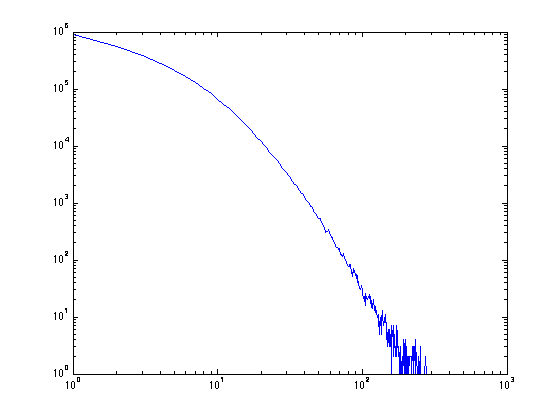
\includegraphics[width=0.5\textwidth]{FIG/cit_result/indegreedist.png} &
     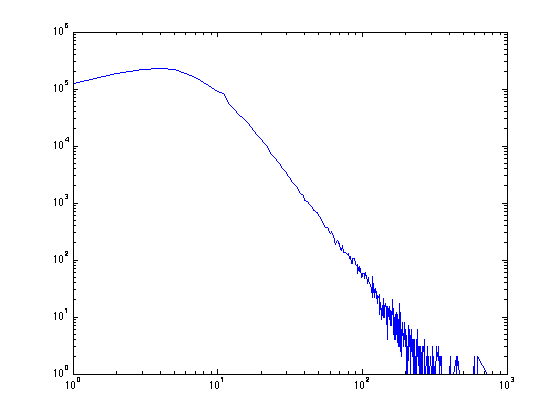
\includegraphics[width=0.5\textwidth]{FIG/cit_result/outdegreedist.png} \\
     %\psfig{figure=FIG/plot.ps,width=2in} \\
     % \psfig{figure=FIG/data.ps,width=2in} &
     % \psfig{figure=FIG/plot.ps,width=2in} \\
    (a) & (b) 
\end{tabular}
\caption{ indegreedist (a) and outdegreedist (b) of cit-Patents}
\label{fig:results}
\end{center}
\end{figure}

\begin{figure}[htbf]
\begin{center}
\begin{tabular}{cc}
     % uncomment the next lines, and give the right ps files
     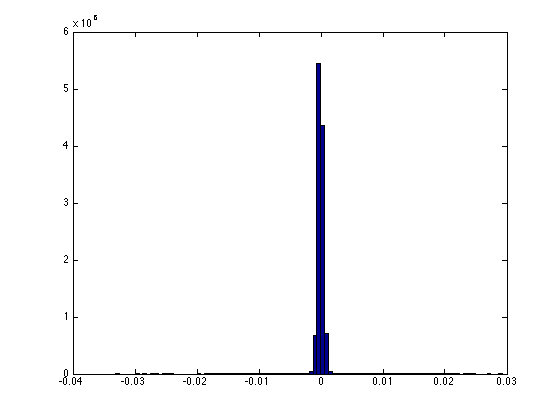
\includegraphics[width=0.5\textwidth]{FIG/cit_result/eigvec.png} &
     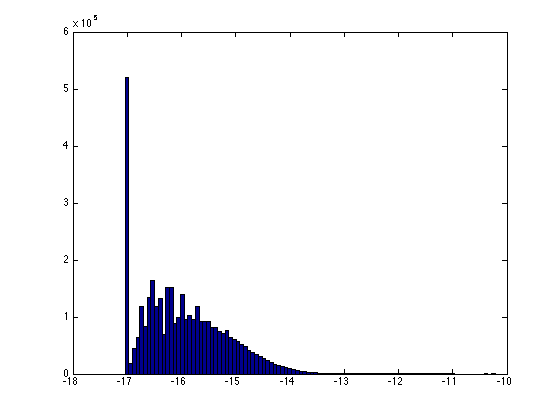
\includegraphics[width=0.5\textwidth]{FIG/cit_result/pagerank.png} \\
     %\psfig{figure=FIG/plot.ps,width=2in} \\
     % \psfig{figure=FIG/data.ps,width=2in} &
     % \psfig{figure=FIG/plot.ps,width=2in} \\
    (a) & (b) 
\end{tabular}
\caption{ eigvec (a) and pagerank (b) of cit-Patents}
\label{fig:results}
\end{center}
\end{figure}

\begin{figure}[htbf]
\begin{center}
\begin{tabular}{cc}
     % uncomment the next lines, and give the right ps files
     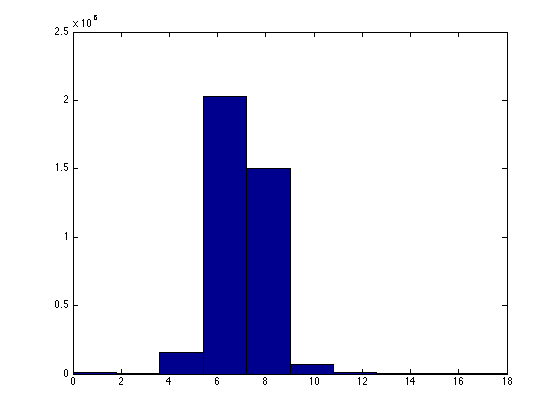
\includegraphics[width=0.5\textwidth]{FIG/cit_result/radius.png} \\
     %\psfig{figure=FIG/plot.ps,width=2in} \\
     % \psfig{figure=FIG/data.ps,width=2in} &
     % \psfig{figure=FIG/plot.ps,width=2in} \\
\end{tabular}
\caption{ radius of cit-Patents}
\label{fig:results}
\end{center}
\end{figure}

\begin{figure}[htbf]
\begin{center}
\begin{tabular}{cc}
     % uncomment the next lines, and give the right ps files
     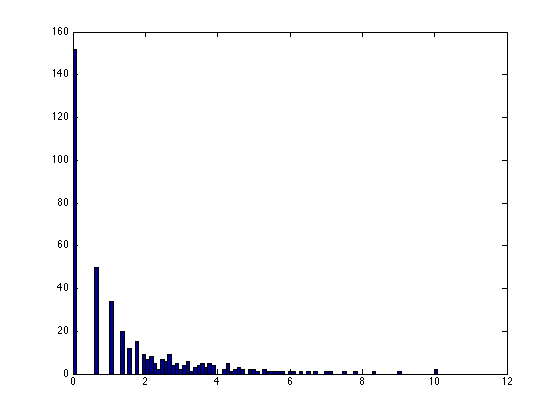
\includegraphics[width=0.5\textwidth]{FIG/soc_result/indegreedist.png} &
     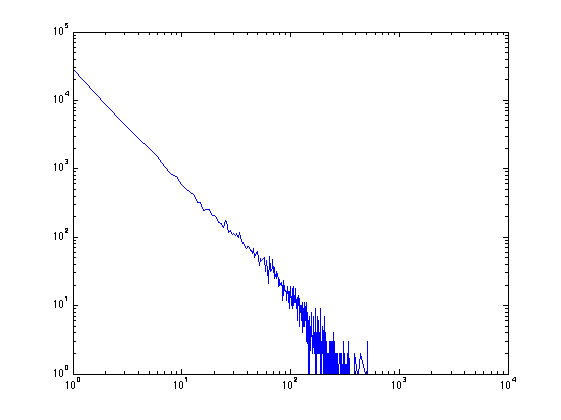
\includegraphics[width=0.5\textwidth]{FIG/soc_result/outdegreedist.png} \\
     %\psfig{figure=FIG/plot.ps,width=2in} \\
     % \psfig{figure=FIG/data.ps,width=2in} &
     % \psfig{figure=FIG/plot.ps,width=2in} \\
    (a) & (b) 
\end{tabular}
\caption{ indegreedist (a) and outdegreedist (b) of soc-Epinions1}
\label{fig:results}
\end{center}
\end{figure}

\begin{figure}[htbf]
\begin{center}
\begin{tabular}{cc}
     % uncomment the next lines, and give the right ps files
     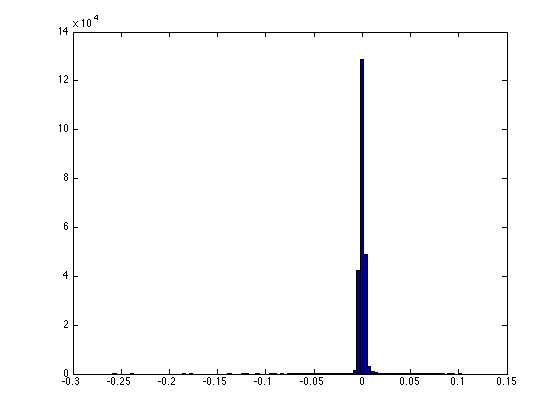
\includegraphics[width=0.5\textwidth]{FIG/soc_result/eigvec.png} &
     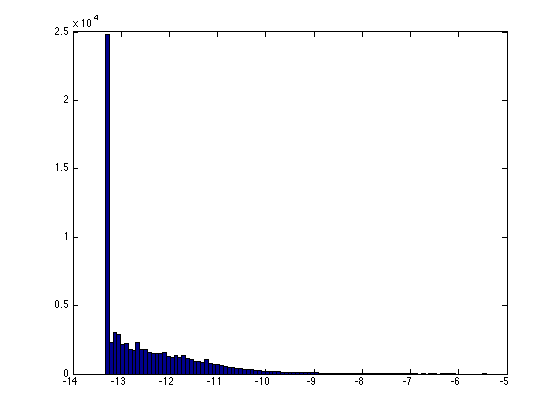
\includegraphics[width=0.5\textwidth]{FIG/soc_result/pagerank.png} \\
     %\psfig{figure=FIG/plot.ps,width=2in} \\
     % \psfig{figure=FIG/data.ps,width=2in} &
     % \psfig{figure=FIG/plot.ps,width=2in} \\
    (a) & (b) 
\end{tabular}
\caption{ eigvec (a) and pagerank (b) of soc-Epinions1}
\label{fig:results}
\end{center}
\end{figure}

\begin{figure}[htbf]
\begin{center}
\begin{tabular}{cc}
     % uncomment the next lines, and give the right ps files
     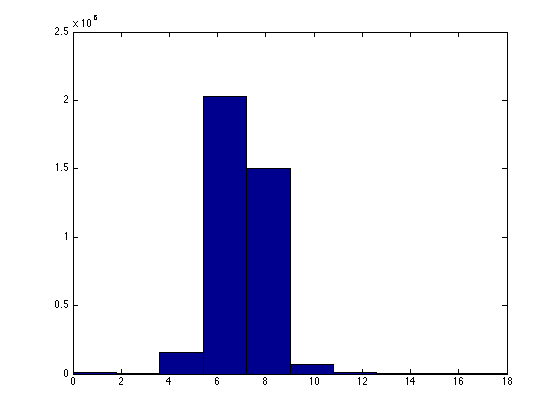
\includegraphics[width=0.5\textwidth]{FIG/cit_result/radius.png} \\
     %\psfig{figure=FIG/plot.ps,width=2in} \\
     % \psfig{figure=FIG/data.ps,width=2in} &
     % \psfig{figure=FIG/plot.ps,width=2in} \\
\end{tabular}
\caption{ radius of soc-Epinions1}
\label{fig:results}
\end{center}
\end{figure}